\chapter{شبیه‌سازی الگوریتم‌ها} \label{ch4}

در این بخش، چهار الگوریتم شبیه‌سازی و تست شده‌اند: الگوریتم \lr{A*} سنتی، الگوریتم \lr{A*} با فاصله توسعه، الگوریتم \lr{A*} دوطرفه با فاصله توسعه، و الگوریتم \lr{EBS-A*}.

\begin{figure}[H]
	\centering
	\begin{subfigure}{0.48\linewidth}
		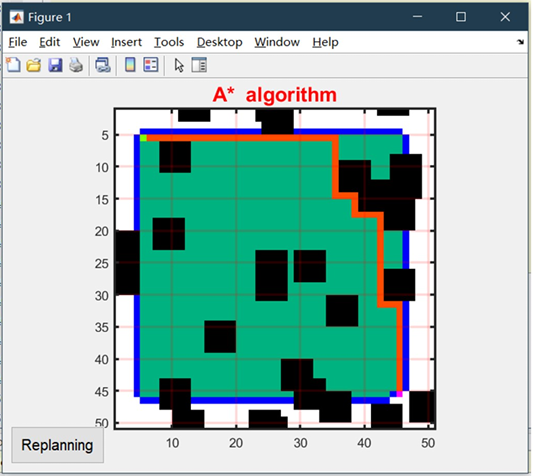
\includegraphics[width=\linewidth]{501}
		\subcaption{زمان سپری شده   \lr{۳۶٫۸۰۵۵۸۴} ثانیه. \\مسیر پیدا شد!\\ تعداد گره‌ها = ۷۹\\ گره گسترش‌یافته = ۱۳۷۲\\ الگوریتم \lr{A*}}\label{501}
	\end{subfigure}
	\begin{subfigure}{0.48\textwidth}
		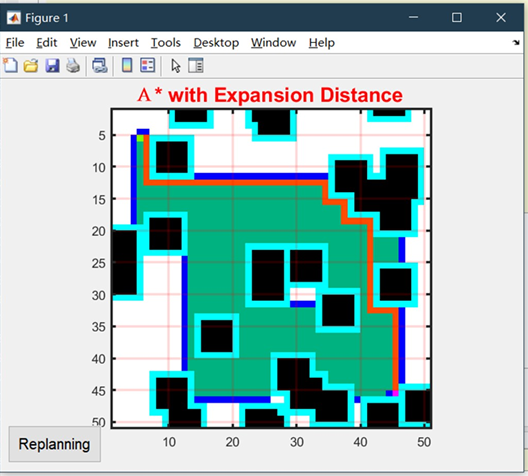
\includegraphics[width=\linewidth]{502}
		\subcaption{زمان سپری شده  \lr{۲۱٫۳۳۶۴۸۷ } ثانیه. \\مسیر پیدا شد! \\تعداد گره‌ها = ۷۹\\ گره گسترش‌یافته = ۷۸۷\\ \lr{A*} با فاصله توسعه}\label{502}
	\end{subfigure}
	\begin{subfigure}{0.48\textwidth}
		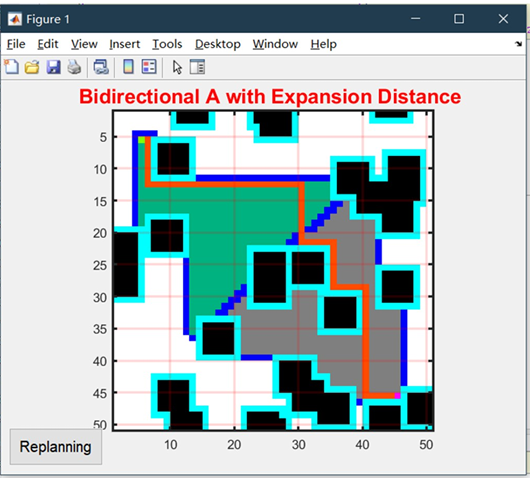
\includegraphics[width=\linewidth]{503}
		\subcaption{مسیر پیدا شد! \\زمان سپری شده \lr{۱۴٫۷۹۳۰۳۸ } ثانیه. \\تعداد گره‌ها = ۷۹\\ گره گسترش‌یافته = ۶۷۹\\\ \lr{A*} دوطرفه با فاصله توسعه}\label{503a}
	\end{subfigure}	
	\begin{subfigure}{0.48\textwidth}
		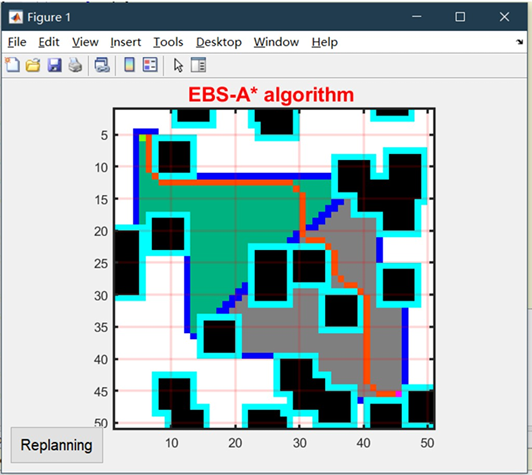
\includegraphics[width=\linewidth]{504}
		\subcaption{مسیر پیدا شد! \\زمان سپری شده \lr{۱۵٫۴۱۱۷۵۸  }ثانیه. \\تعداد گره‌ها = ۶۶\\ گره گسترش‌یافته = ۶۸۲\\ الگوریتم \lr{EBS-A*}}\label{503b}
	\end{subfigure}	
	\caption{نتایج شبیه‌سازی چهار الگوریتم روی یک نقشه ۵۰ در ۵۰.}
	\label{p3}
\end{figure}
 مقیاس نقشه در آزمایش شبیه‌سازی \lr{50×50} است و اندازه هر مانع در نقشه \lr{5×5} می‌باشد. موقعیت موانع به‌طور تصادفی بر اساس نقطه مرکز روی نقشه تولید می‌شود. چهار الگوریتم تست شده‌اند و نتایج برنامه‌ریزی مسیر در شکل \ref{p3} نشان داده شده است.
بررسی عملکرد چهار الگوریتم مسیریابی در نقشه‌های با ابعاد \lr{50×50} نشان‌دهنده برتری قابل‌توجه الگوریتم \lr{EBS-A*} در شاخص‌های کلیدی است:

\begin{itemize}
	\item سرعت و کارایی: سرعت اجرای الگوریتم \lr{EBS-A*} نسبت به \lr{A*} سنتی حدود \lr{۳۲۸\%} بهبود یافته و زمان اجرای آن تنها معادل \lr{۲۶٫۴۸\%} زمان الگوریتم \lr{A*} سنتی است.
	
	\item همواری مسیر: \lr{EBS-A*} با حذف کامل چرخش‌های زاویه قائمه (تعداد صفر در برابر \lr{۷} چرخش در \lr{A*}) و کاهش بیشترین زاویه چرخش از \lr{۹۰} به \lr{۴۵}، مسیر بسیار نرم‌تر و پایدارتری ایجاد می‌کند.
	
	\item طول مسیر و ایمنی: این الگوریتم به کمترین تعداد گره برای برنامه‌ریزی مسیر نیاز دارد و تعداد گره‌های بحرانی (مجاور موانع) را از \lr{۳۷} گره در \lr{A*} سنتی به تنها \lr{۳} گره کاهش داده است.
	
	\item گره‌های توسعه: تعداد گره‌های توسعه در این الگوریتم به \lr{۶۸۲} مورد کاهش یافته که نشان‌دهنده کارایی بالای جستجو است.
	
	\item این نتایج هم در یک نقشه ثابت (جدول \ref{50}) و هم به صورت میانگین در نقشه‌های تصادفی (جدول \ref{r50}) تأیید شده‌اند.
	
	\begin{table}[H]
		\centering
		\caption{ نتایج شبیه‌سازی چهار الگوریتم روی نقشه \lr{۵۰×۵۰} }
		\setlength{\arrayrulewidth}{1pt}
		\setlength{\tabcolsep}{10pt}
		\renewcommand{\arraystretch}{1.5}
		\rowcolors{1}{blue!20}{white}
		\resizebox{\textwidth}{!}{%
		\begin{tabular}{|c!{\color{blue}\vrule width 2pt}c|c|c|c|}
			\hline 
			شاخص‌ها & الگوریتم \lr{A*} & \lr{A*} با فاصله توسعه & \lr{A*} دوطرفه با فاصله توسعه & الگوریتم \lr{EBS-A*} \\
			\noalign{\global\setlength{\arrayrulewidth}{2pt}}\hline\noalign{\global\setlength{\arrayrulewidth}{0.4pt}}
			زمان اجرا (ثانیه) & \lr{۳۶٫۸۰۶(۱۰۰\%)} & \lr{۲۱٫۷۸۲(۵۹٫۱۸\%)} & \lr{۹٫۶۳۷(۲۶٫۱۸\%)} & \lr{۹٫۷۴۷(۲۶٫۴۸\%)} \\
			\hline 
			تعداد گره‌ها & \lr{۷۹} & \lr{۷۹} & \lr{۷۹} & \lr{۶۶} \\
			\hline
			تعداد گردش‌های ۹۰ درجه & \lr{۷} & \lr{۹} & \lr{۸} & \lr{۰} \\
			\hline
			حداکثر زاویه چرخش & \lr{۹۰°} & \lr{۹۰°} & \lr{۹۰°} & \lr{۴۵°} \\
			\hline
			تعداد گره‌های گسترش‌یافته & \lr{۱،۳۷۲} & \lr{۷۸۷} & \lr{۶۷۹} & \lr{۶۸۲} \\
			\hline
			تعداد گره‌های بحرانی & \lr{۳۷} & \lr{۰} & \lr{۰} & \lr{۳} \\
			\hline
		\end{tabular}}
		\label{50}
	\end{table}
	
	\begin{table}[H]
		\centering
		\caption{ میانگین نتایج شبیه‌سازی چهار الگوریتم روی نقشه تصادفی  \lr{۵۰×۵۰} }
		\setlength{\arrayrulewidth}{1pt}
		\setlength{\tabcolsep}{10pt}
		\renewcommand{\arraystretch}{1.5}
		\rowcolors{1}{blue!20}{white}
		\resizebox{\textwidth}{!}{%
		\begin{tabular}{|c!{\color{blue}\vrule width 2pt}c|c|c|c|}
			\hline 
			شاخص‌ها & الگوریتم \lr{A*} & \lr{A*} با فاصله توسعه & \lr{A*} دوطرفه با فاصله توسعه & الگوریتم \lr{EBS-A*} \\
			\noalign{\global\setlength{\arrayrulewidth}{2pt}}\hline\noalign{\global\setlength{\arrayrulewidth}{0.4pt}}
			زمان اجرا (ثانیه) & \lr{۳۳٫۵۵۹(۱۰۰\%)} & \lr{۲۱٫۳۸۶(۶۳٫۷۳\%)} & \lr{۵٫۶۳۹(۱۶٫۸۰\%)} & \lr{۷٫۸۳۵(۲۳٫۳۵\%)} \\
			\hline 
			تعداد گره‌ها & \lr{۷۹٫۴} & \lr{۷۹٫۴} & \lr{۷۹٫۴} & \lr{۶۷} \\
			\hline
			تعداد گردش‌های ۹۰ درجه & \lr{۶٫۴} & \lr{۶٫۲} & \lr{۷} & \lr{۰} \\
			\hline
			حداکثر زاویه چرخش & \lr{۹۰°} & \lr{۹۰°} & \lr{۹۰°} & \lr{۴۵°} \\
			\hline
			تعداد گره‌های گسترش‌یافته & \lr{۱،۰۸۵} & \lr{۷۴۴٫۸} & \lr{۵۵۳} & \lr{۶۹۳٫۸} \\
			\hline
			تعداد گره‌های بحرانی & \lr{۳۶٫۲} & \lr{۰} & \lr{۰} & \lr{۳} \\
			\hline
		\end{tabular}}
		\label{r50}
	\end{table}
	
\end{itemize}

\newpage
نتایج برنامه‌ریزی مسیر نقشه \lr{۱۰۰ × ۱۰۰} در شکل \ref{p4} نشان داده شده است.

\begin{figure}[H]
	\centering
	\begin{subfigure}{0.48\linewidth}
		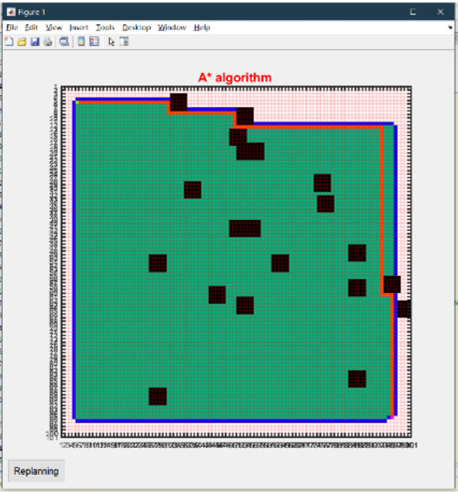
\includegraphics[width=\linewidth]{1001}
		\subcaption{زمان سپری شده   \lr{۳۶٫۸۰۵۵۸۴} ثانیه. \\مسیر پیدا شد!\\ تعداد گره‌ها = ۷۹\\ گره گسترش‌یافته = ۱۳۷۲\\ الگوریتم \lr{A*}}\label{1001}
	\end{subfigure}
	\begin{subfigure}{0.48\textwidth}
		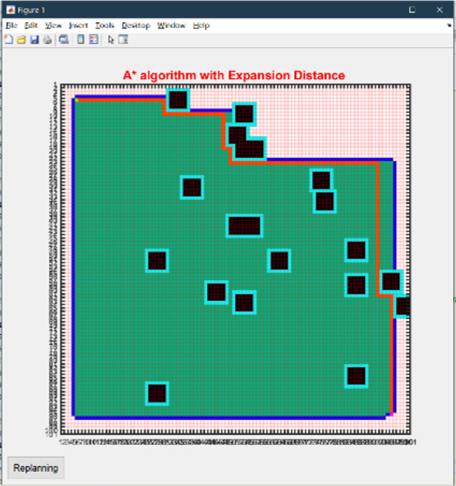
\includegraphics[width=\linewidth]{1002}
		\subcaption{زمان سپری شده  \lr{۲۱٫۳۳۶۴۸۷ } ثانیه. \\مسیر پیدا شد! \\تعداد گره‌ها = ۷۹\\ گره گسترش‌یافته = ۷۸۷\\ \lr{A*} با فاصله توسعه}\label{1002}
	\end{subfigure}
	\begin{subfigure}{0.48\textwidth}
		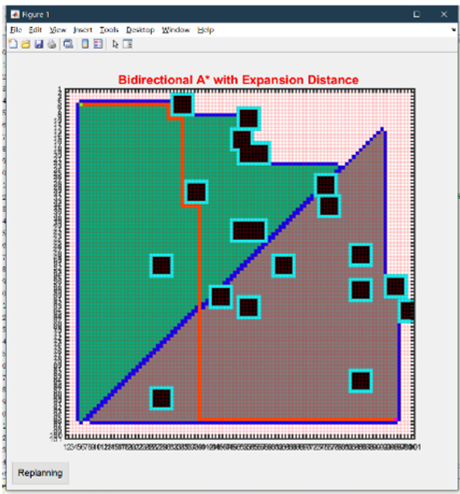
\includegraphics[width=\linewidth]{1003}
		\subcaption{مسیر پیدا شد! \\زمان سپری شده \lr{۱۴٫۷۹۳۰۳۸ } ثانیه. \\تعداد گره‌ها = ۷۹\\ گره گسترش‌یافته = ۶۷۹\\\ \lr{A*} دوطرفه با فاصله توسعه}\label{1003}
	\end{subfigure}	
	\begin{subfigure}{0.48\textwidth}
		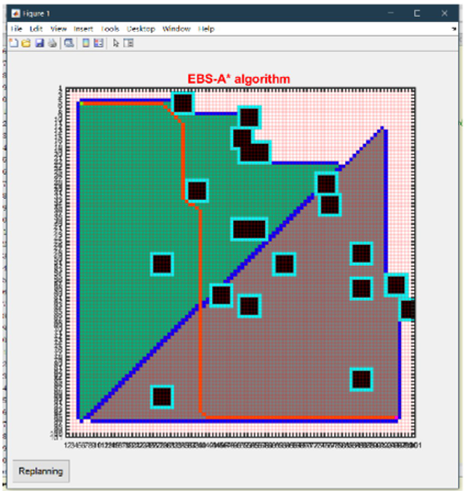
\includegraphics[width=\linewidth]{1004}
		\subcaption{مسیر پیدا شد! \\زمان سپری شده \lr{۱۵٫۴۱۱۷۵۸  }ثانیه. \\تعداد گره‌ها = ۶۶\\ گره گسترش‌یافته = ۶۸۲\\ الگوریتم \lr{EBS-A*}}\label{1004}
	\end{subfigure}	
	\caption{نتایج شبیه‌سازی چهار الگوریتم روی یک نقشه ۱۰۰ در ۱۰۰.}
	\label{p4}
\end{figure}

نتایج آماری برای نقشه‌ی واحد در جدول \ref{100} و برای نقشه‌های تصادفی در جدول \ref{r100} آمده است.

\begin{table}[H]
	\centering
	\caption{ نتایج شبیه‌سازی چهار الگوریتم روی نقشه \lr{۱۰۰×۱۰۰}}
	\setlength{\arrayrulewidth}{1pt}
	\setlength{\tabcolsep}{10pt}
	\renewcommand{\arraystretch}{1.5}
	\rowcolors{1}{blue!20}{white}
	\resizebox{\textwidth}{!}{%
	\begin{tabular}{|c!{\color{blue}\vrule width 2pt}c|c|c|c|}
		\hline 
		شاخص‌ها & الگوریتم \lr{A*} & \lr{A*} با فاصله توسعه & \lr{A*} دوطرفه با فاصله توسعه & الگوریتم \lr{EBS-A*} \\
		\noalign{\global\setlength{\arrayrulewidth}{2pt}}\hline\noalign{\global\setlength{\arrayrulewidth}{0.4pt}}
		زمان اجرا (ثانیه) & \lr{۳۰۲٫۴۶۷} & \lr{۲۷۱٫۱۹۰} & \lr{۱۳۴٫۷۱۹} & \lr{۱۳۸٫۸۱۳} \\
		\hline 
		تعداد گره‌ها & \lr{۱۷۹} & \lr{۱۷۹} & \lr{۱۷۹} & \lr{۱۶۷} \\
		\hline
		تعداد گردش‌های ۹۰ درجه & \lr{۷} & \lr{۹} & \lr{۶} & \lr{۰} \\
		\hline
		حداکثر زاویه چرخش & \lr{۹۰°} & \lr{۹۰°} & \lr{۹۰°} & \lr{۴۵°} \\
		\hline
		تعداد گره‌های گسترش‌یافته & \lr{۷،۵۰۹} & \lr{۶،۷۲۲} & \lr{۶،۵۳۱} & \lr{۶،۵۳۳} \\
		\hline
		تعداد گره‌های بحرانی & \lr{۳۱} & \lr{۰} & \lr{۰} & \lr{۲} \\
		\hline
	\end{tabular}}
	\label{100}
\end{table}


\begin{table}[H]
	\centering
	\caption{ میانگین نتایج شبیه‌سازی چهار الگوریتم روی نقشه تصادفی \lr{۱۰۰×۱۰۰}}
	\setlength{\arrayrulewidth}{1pt}
	\setlength{\tabcolsep}{10pt}
	\renewcommand{\arraystretch}{1.5}
	\rowcolors{1}{blue!20}{white}
	\resizebox{\textwidth}{!}{%
	\begin{tabular}{|c!{\color{blue}\vrule width 2pt}c|c|c|c|}
		\hline 
		شاخص‌ها & الگوریتم \lr{A*} & \lr{A*} با فاصله توسعه & \lr{A*} دوطرفه با فاصله توسعه & الگوریتم \lr{EBS-A*} \\
		\noalign{\global\setlength{\arrayrulewidth}{2pt}}\hline\noalign{\global\setlength{\arrayrulewidth}{0.4pt}}
		زمان اجرا (ثانیه) & \lr{۲۶۹٫۳۳۵} & \lr{۲۶۸٫۳۳۱} & \lr{۱۲۸٫۷۷۵} & \lr{۱۲۵٫۶۷۷} \\
		\hline 
		تعداد گره‌ها & \lr{۱۷۹} & \lr{۱۷۹} & \lr{۱۷۹} & \lr{۱۷۰٫۸} \\
		\hline
		تعداد گردش‌های ۹۰ درجه & \lr{۶} & \lr{۵٫۷} & \lr{۶} & \lr{۰} \\
		\hline
		حداکثر زاویه چرخش & \lr{۹۰°} & \lr{۹۰°} & \lr{۹۰°} & \lr{۴۵°} \\
		\hline
		تعداد گره‌های گسترش‌یافته & \lr{۷،۷۰۹٫۴} & \lr{۷،۳۰۲٫۸} & \lr{۶،۸۱۷٫۴} & \lr{۶،۵۹۹} \\
		\hline
		تعداد گره‌های بحرانی & \lr{۱۰} & \lr{۰} & \lr{۰} & \lr{۲} \\
		\hline
	\end{tabular}}
	\label{r100}
\end{table}

نتایج برنامه‌ریزی مسیر نقشه \lr{۱۵۰ × ۱۵۰} در شکل زیر نشان داده شده است.

\begin{figure}[H]
	\centering
	\begin{subfigure}{0.48\linewidth}
		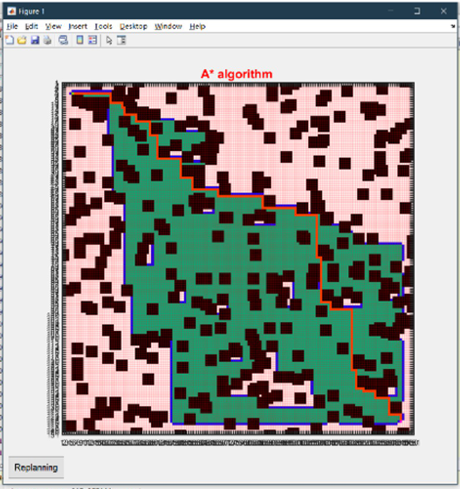
\includegraphics[width=\linewidth]{1501}
		\subcaption{زمان سپری شده   \lr{۳۶٫۸۰۵۵۸۴} ثانیه. \\مسیر پیدا شد!\\ تعداد گره‌ها = ۷۹\\ گره گسترش‌یافته = ۱۳۷۲\\ الگوریتم \lr{A*}}\label{1501}
	\end{subfigure}
	\begin{subfigure}{0.48\textwidth}
		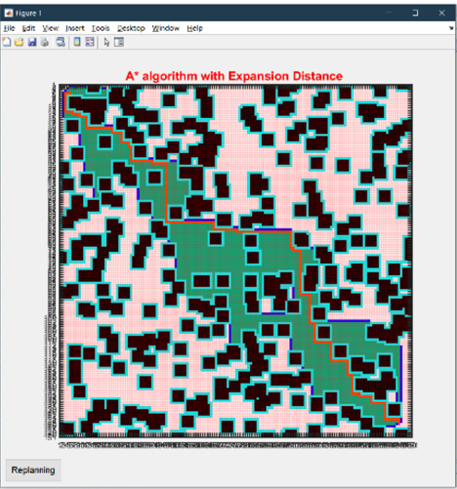
\includegraphics[width=\linewidth]{1502}
		\subcaption{زمان سپری شده  \lr{۲۱٫۳۳۶۴۸۷ } ثانیه. \\مسیر پیدا شد! \\تعداد گره‌ها = ۷۹\\ گره گسترش‌یافته = ۷۸۷\\ \lr{A*} با فاصله توسعه}\label{1502}
	\end{subfigure}
	\begin{subfigure}{0.48\textwidth}
		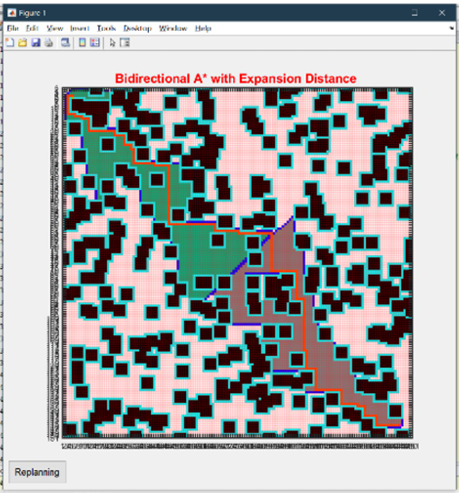
\includegraphics[width=\linewidth]{1503}
		\subcaption{مسیر پیدا شد! \\زمان سپری شده \lr{۱۴٫۷۹۳۰۳۸ } ثانیه. \\تعداد گره‌ها = ۷۹\\ گره گسترش‌یافته = ۶۷۹\\\ \lr{A*} دوطرفه با فاصله توسعه}\label{1503}
	\end{subfigure}	
	\begin{subfigure}{0.48\textwidth}
		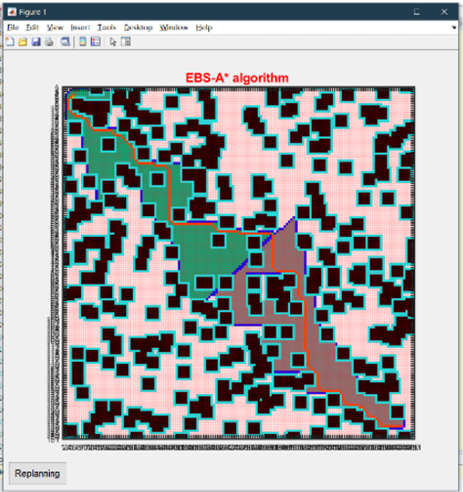
\includegraphics[width=\linewidth]{1504}
		\subcaption{مسیر پیدا شد! \\زمان سپری شده \lr{۱۵٫۴۱۱۷۵۸  }ثانیه. \\تعداد گره‌ها = ۶۶\\ گره گسترش‌یافته = ۶۸۲\\ الگوریتم \lr{EBS-A*}}\label{1504}
	\end{subfigure}	
	\caption{نتایج شبیه‌سازی چهار الگوریتم روی یک نقشه ۱۵۰ در ۱۵۰.}
	\label{p5}
\end{figure}



نتایج آماری برای نقشه‌ی واحد و نقشه‌های تصادفی در جداول زیر آمده است.



\begin{table}[H]
	\centering
	\caption{ نتایج شبیه‌سازی چهار الگوریتم روی نقشه \lr{۱۵۰×۱۵۰}}
	\setlength{\arrayrulewidth}{1pt}
	\setlength{\tabcolsep}{10pt}
	\renewcommand{\arraystretch}{1.5}
	\rowcolors{1}{blue!20}{white}
	\resizebox{\textwidth}{!}{%
	\begin{tabular}{|c!{\color{blue}\vrule width 2pt}c|c|c|c|}
		\hline 
		شاخص‌ها & الگوریتم \lr{A*} & \lr{A*} با فاصله توسعه & \lr{A*} دوطرفه با فاصله توسعه & الگوریتم \lr{EBS-A*} \\
		\noalign{\global\setlength{\arrayrulewidth}{2pt}}\hline\noalign{\global\setlength{\arrayrulewidth}{0.4pt}}
		زمان اجرا (ثانیه) & \lr{۲۶۷٫۳۷۷} & \lr{۱۰۰٫۵۹۷} & \lr{۵۶٫۷۵۵} & \lr{۵۶٫۸۶۶} \\
		\hline 
		تعداد گره‌ها & \lr{۲۷۹} & \lr{۲۸۵} & \lr{۲۸۵} & \lr{۲۲۸} \\
		\hline
		تعداد گردش‌های ۹۰ درجه & \lr{۳۹} & \lr{۴۷} & \lr{۴۲} & \lr{۰} \\
		\hline
		حداکثر زاویه چرخش & \lr{۹۰°} & \lr{۹۰°} & \lr{۹۰°} & \lr{۴۵°} \\
		\hline
		تعداد گره‌های گسترش‌یافته & \lr{۷،۴۳۷} & \lr{۲،۹۳۱} & \lr{۲،۶۳۳} & \lr{۲،۶۴۴} \\
		\hline
		تعداد گره‌های بحرانی & \lr{۱۹۲} & \lr{۰} & \lr{۰} & \lr{۱۱} \\
		\hline
	\end{tabular}}
	\label{150}
\end{table}


\begin{table}[H]
	\centering
	\caption{ میانگین نتایج شبیه‌سازی چهار الگوریتم روی نقشه تصادفی \lr{۱۵۰×۱۵۰}}
	\setlength{\arrayrulewidth}{1pt}
	\setlength{\tabcolsep}{10pt}
	\renewcommand{\arraystretch}{1.5}
	\rowcolors{1}{blue!20}{white}
	\resizebox{\textwidth}{!}{%
	\begin{tabular}{|c!{\color{blue}\vrule width 2pt}c|c|c|c|}
		\hline 
		شاخص‌ها & الگوریتم \lr{A*} & \lr{A*} با فاصله توسعه & \lr{A*} دوطرفه با فاصله توسعه & الگوریتم \lr{EBS-A*} \\
		\noalign{\global\setlength{\arrayrulewidth}{2pt}}\hline\noalign{\global\setlength{\arrayrulewidth}{0.4pt}}
		زمان اجرا (ثانیه) & \lr{۲۶۴٫۷۸۹} & \lr{۱۱۶٫۳۷۹} & \lr{۴۵٫۳۸۱} & \lr{۵۷٫۰۳۲} \\
		\hline 
		تعداد گره‌ها & \lr{۲۷۹٫۴} & \lr{۲۸۴٫۲} & \lr{۲۸۳٫۸} & \lr{۲۳۳٫۴} \\
		\hline
		تعداد گردش‌های ۹۰ درجه & \lr{۲۹} & \lr{۲۶٫۲} & \lr{۲۸} & \lr{۰} \\
		\hline
		حداکثر زاویه چرخش & \lr{۹۰°} & \lr{۹۰°} & \lr{۹۰°} & \lr{۴۵°} \\
		\hline
		تعداد گره‌های گسترش‌یافته & \lr{۸،۸۶۴٫۴} & \lr{۳،۷۱۳٫۲} & \lr{۲،۷۱۳} & \lr{۳،۳۲۵٫۶} \\
		\hline
		تعداد گره‌های بحرانی & \lr{۲۰۱} & \lr{۰} & \lr{۰} & \lr{۱۲} \\
		\hline
	\end{tabular}}
	\label{r150}
\end{table}

اما کارایی الگوریتم \lr{A*} برابر با \lr{۴٫۷} برابر الگوریتم \lr{A*} است. دلیل این امر این است که در نقشه \lr{۱۰۰×۱۰۰} موانع کمی وجود دارد، اما در نقشه \lr{۱۵۰×۱۵۰} موانع متراکم وجود دارند. در محیطی با موانع متراکم، کارایی الگوریتم بیشتر است.

